\documentclass[10pt]{article}

\usepackage{parskip}
\usepackage[margin=1in]{geometry} 
\usepackage{tikz}
\usetikzlibrary{positioning}
\usepackage{amsmath,amsthm,amssymb, graphicx, multicol, array}
\usepackage{enumitem}
\usepackage{amssymb}
\usepackage{float}
\usepackage{href-ul}
 
\newcommand{\N}{\mathbb{N}}
\newcommand{\Z}{\mathbb{Z}}
 
\newenvironment{problem}[2][Problem]{\begin{trivlist}
\item[\hskip \labelsep {\bfseries #1}\hskip \labelsep {\bfseries #2.}]}{\end{trivlist}}

\begin{document}
 
\title{Instrumental Variables}
\author{Jakob Sverre Alexandersen\\
GRA4158 Marketing and the Analysis of Experiments and Quasi-Experiments\\
Lecture 7}
\maketitle

\tableofcontents
\newpage

\section{Non-random assignment}
\begin{itemize}
    \item We are now moving quasi-experimental or observational 
    \begin{itemize}
        \item We typically do not have random assignment 
        \item Or at least we do not have full compliance with random assignment
    \end{itemize}
    \item We still want to estimate causal effects 
    \item What are ways of identifying causal effects from non-randomized data?
    \item We will allow the treatment variable to be continuous/metric (not just discrete: treatment and control)
\end{itemize}
\section{Recap: fundamental assumption of OLS}
\begin{itemize}
    \item Let's assume a linear regression equation on the form 
    \begin{gather*}
        Y = \alpha + \beta X + u
    \end{gather*}
    \item A fundamental assumption for the unbiasedness of the regression coefficients $\beta $ is the independence of the model error $u $ from the regressors $X $,
    \begin{itemize}
        \item i.e., EV of the error is not a function of $X $: 
        \begin{gather*}
            \mathbb{E}[u|X] = \mathbb{E}[u] = 0
        \end{gather*}
    \end{itemize}
    \item Whenever this assumption is violated, we have $\text{cov}(u, X)\neq 0 $
    \begin{itemize}
        \item i.e., a covariance/correlation between predictor(s) and model error term 
        \item This problem is often termed ``endogeneity''
        \item Variables $X $ for which $\mathbb{E}[u|x] \neq \mathbb{E}[u] = 0 $ are called ``endogenous variables''
        \item The parameter estimate $\hat{\beta}$ of endogenous variables does not allow a causal interpretation
    \end{itemize}
    \item \textbf{If we omit variables from a multivariate model when we estimate, we will get a biased and inconsistent estimate}
\end{itemize}
\newpage 
\section{Long vs. short regression}
\begin{itemize}
    \item Long regression (i.e., complete specification): $Y = \alpha + \beta_1X_1 + \beta_2X_2 + u $
    \item Short regression (i.e., omitted variables): $Y = \alpha + \beta_1' X_1 + u $
    \item Because $\mathbb{E}[v|x_1] \neq 0 $ the coefficient estimate $\beta_1'\neq \beta_1 $, when cov($X_1, X_2) \neq 0 \text{ and }\beta_2\neq 0 $
    \begin{itemize}
        \item That is why the parameter estimate of endogenous variables does not allow a causal interpretation, because it does not equal the ``true'' population parameter
    \end{itemize}
\end{itemize}
\section{Some other potential causes for endogeneity}
\begin{itemize}
    \item Measurement error
    \begin{itemize}
        \item Predictors are measured with error 
        \item Measurement errors are correlated 
    \end{itemize}
    \item Simultaneity
    \begin{itemize}
        \item $X \text{ and } Y $ are determined simultaneously (i.e., they cause each other)
    \end{itemize}
    \item Before starting to do any (endogeneity) correction, we should make sure that we have done our best to rule out these potential problems 
    \begin{itemize}
        \item Endogeneity correction using instrumental variables should be left for what we are not able to correct; e.g., by uncluding relevant control variables, etc. 
    \end{itemize}
\end{itemize}
\section{Instrumental variables (IV)}
\begin{itemize}
    \item Basic idea: 
    \begin{itemize}
        \item $X_1 $ is (never) perfectly correlated with $v $, thus, there is variance in $X_1 $ that is uncorrelated with $v $
        \item Split the endogenous predictor variable $X_1 $ into two parts 
        \begin{itemize}
            \item One that is correlated with the error term (the one that causes $\mathbb{E}[v|x_1] \neq 0 $)
            \item One that is uncorrelated with the error term 
        \end{itemize}
        \item Use the uncorrelated part of $X_1 $ to estimate a consistent effect of $X_1 $ on $Y $
    \end{itemize}
    \item How to do the split?
    \begin{itemize}
        \item We can utilize an IV $Z $
        \item Must fulfill two important assumptions 
        \begin{enumerate}
            \item Instrument relevance: $\text{cov}(X_1, Z) \neq 0 $
            \item Instrument exogeneity: $\text{cov}(Z, v) = 0 $
        \end{enumerate}
    \end{itemize}
\end{itemize}
\newpage 
\section{How to estimate the model: 2SLS}
\begin{itemize}
    \item A typical approach to utilizing IVs is two stage least squares (2SLS)
    \item First stage: 
    \begin{itemize}
        \item Regress $X_1 $ on $Z $ and obtain predicted values $\hat{X}_1 = \alpha + \gamma_1 Z $
        \item This requires that $\gamma_1 \neq 0 \text{ i.e., cov}(X_1, Z) \neq 0 $
        \item If $\text{cov}(Z, v) = 0,\, \hat{X} $ contains only variation in $X_1 $ that is related to $Z $ and thus unrelated with $v $
    \end{itemize}
    \item Second stage: 
    \begin{itemize}
        \item Use these predicted $\hat{X}_1 $ to estimate the effect of $X_1\text{ on } Y $
        \item Estimate: $Y = \alpha + \beta_1\hat{X}_1 + v $
    \end{itemize}
    \item Depending on the quality of $Z $, the estimated effect $\hat{\beta}_1 $ should approach $\beta_1 $ from the long regression 
\end{itemize}
\section{IV assumptions}
\begin{itemize}
    \item The relevance condition: 
    \begin{itemize}
        \item $X_1 $ must be correlated with $Z $
        \item This can be tested by regressing $X_1 $ on $Z $ obtaining $\gamma_1 $
        \item In practice, the correlation should be strong 
    \end{itemize}
    \item The exogeneity condition (exclusion restriction): 
    \begin{itemize}
        \item $Z $ must be uncorrelated with the model error term $v $
        \item Affects the outcome $Y $ only through the endogenous variable $X_1 $
        \begin{itemize}
            \item i.e., there is no direct effect of $Z \text{ on } Y $
            \item i.e., $Y \bot Z|X_1 $
        \end{itemize}
    \end{itemize}
\end{itemize}
\newpage 
\subsection{The exogeneity condition / exclusion restriction}
\begin{figure}[H]
    \centering
    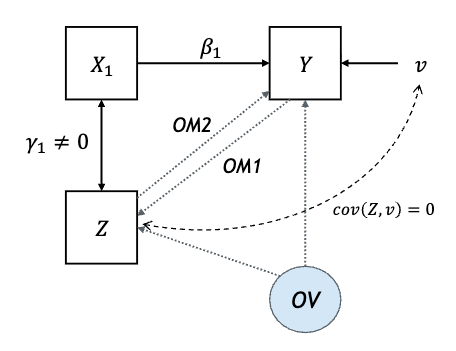
\includegraphics[width=0.5\textwidth]{2026-02-25-18-53-44.png}
\end{figure}
\begin{itemize}
    \item The exogeneity condition has three implications:
    \begin{itemize}
        \item No OM1: no omitted mechanisms enabling the IV to affect the dependent variable directly or indirectly that is not through $X_1 $
        \item No OM2: no omitted mechanisms enabling the dependent variable to affect the IV (i.e., and form of reverse-causality)
        \item No OVs: no omitted variables affecting both the IV and the dependent variable 
    \end{itemize}
    \item These assumptions are usually not testable, but require careful judgement by the researcher 
\end{itemize}

\end{document}